%   Borrowed from A. Shafiei
%
%   Copyright (c)  2023  A. Shafiei
%   Permission is granted to copy, distribute and/or modify this document
%    under the terms of the GNU Free Documentation License, Version 1.3
%    or any later version published by the Free Software Foundation;
%    with no Invariant Sections, no Front-Cover Texts, and no Back-Cover Texts.
%    A copy of the license is included in the section entitled "GNU
%    Free Documentation License".

\documentclass[
    aspectratio=169,
    dvipsnames,
    svgnames,
    x11names
]{beamer}

% URLs and hyperlinks ---------------------------------------
\usepackage{hyperref}
\hypersetup{
    colorlinks=true,
    linkcolor=NavyBlue,
    filecolor=magenta,      
    urlcolor=blue,
}
\usepackage{xurl}
%---------------------------------------------------

\usefonttheme{serif}
\usepackage{listings}
\usepackage{docs/style}

\usepackage{xepersian}
\settextfont{Yas}

% Persian specific
\newcommand{\itmsep}[1]{\raggedleft\setlength\itemsep{#1}}
\newcommand{\itemr}{\raggedleft\setlength\itemsep{3mm}}
\newcommand{\fn}[2]{{\LR{\footnote[frame,#1]{{~\LR{#2}}}}}}
\newcommand{\fnn}[1]{{\LR{\footnote[frame]{{~\LR{#1}}}}}}
\newcommand{\m}[1]{\ensuremath{\mathnormal{#1}}}
\newcommand{\mc}[1]{\ensuremath{\mathtt{#1}}}
\newcommand{\scl}{\ensuremath{\Sigma^*}\xspace}
\newcommand{\gcl}{\ensuremath{\Gamma^*}\xspace}
\newcommand{\gin}{\ensuremath{\mathnormal{\in}}\xspace}
%\newcommand{\gand}{\ensuremath{\mathnormal{\land}}\xspace}
\newcommand{\gand}{\&\&\xspace}
\newcommand{\alglr}{\LTR\ttfamily\small}
\newcommand{\st}[1]{\ensuremath{\mathnormal{\{#1\}}}\xspace}
\newcommand{\gst}[1]{\ensuremath{\mathnormal{\{\text{\texttt{#1}}\}}}\xspace}
\newcommand{\cpp}{C++\xspace}
\newcommand{\enc}[1]{\ensuremath{\mathnormal{\langle#1\rangle}}\xspace}
\newcommand{\abo}[1]{\ensuremath{\mathnormal{O(#1)}}\xspace}
\newcommand{\aso}[1]{\ensuremath{\mathnormal{o(#1)}}\xspace}
\newcommand{\aom}[1]{\ensuremath{\mathnormal{\Omega(#1)}}\xspace}
\newcommand{\ath}[1]{\ensuremath{\mathnormal{\Theta(#1)}}\xspace}
\newcommand{\dom}[2]{\ensuremath{\mathnormal{\Big[ \dfrac{#1}{#2} \Big]}}\xspace}

\newcommand{\Proc}[2]{\Statex \textbf{procedure} \textsc{#1}(#2)}
\newcommand{\Func}[2]{\Statex \textbf{function} \textsc{#1}(#2)}
\newcommand{\To}{\textbf{to}\xspace}

\newcommand\pro{\ensuremath{\rightarrow}\xspace}
\newcommand\der{\ensuremath{\Rightarrow}\xspace}
\newcommand\ders{\ensuremath{\stackrel{\mbox{*}}{\Rightarrow}}\xspace}
\newcommand{\dern}[1]{\ensuremath{\stackrel{\mbox{\small #1}}{\Rightarrow}}\xspace}
\newcommand\move{\ensuremath{\vdash}\xspace}
\newcommand\moves{\ensuremath{\stackrel{\small *}{\vdash}}\xspace}
\newcommand{\movesn}[1]{\ensuremath{\stackrel{\small *}{\vdash_{#1}}}\xspace}
\newcommand{\moven}[1]{\ensuremath{\mathnormal{\vdash_{#1}}}\xspace}

\newcommand{\code}[1]{{\LR{\texttt{#1}}}}
\newcommand{\txtlr}[1]{\text{\LR{#1}}}


% Abbreviations
\newcommand{\ie}{\latin{i.e.,~}}
\newcommand{\eg}{\latin{e.g.,~}}
\newcommand{\cf}{\latin{cf.~}}
\newcommand{\etal}{\latin{et al.~}}
\newcommand{\etc}{\unskip~\latin{etc.}\xspace}
\newcommand{\apriori}{\latin{a priori}}
\newcommand{\wrt}{\latin{w.r.t.~}}
%\newtheorem{theorem}{Theorem}

\newcommand\NN{\ensuremath{\mathbb{N}}\xspace}
\newcommand\RR{\ensuremath{\mathbb{R}}\xspace}
\newcommand\NNS{\ensuremath{\mathbb{N}^*}\xspace}
\newcommand\NNZ{\ensuremath{\mathbb{N}\backslash\{0\}}\xspace}
\newcommand\RRP{\ensuremath{\mathbb{R}^+}\xspace}
\newcommand\vect[1]{\ensuremath{\boldsymbol{\vec{#1}}}}
\newcommand\MP{\ensuremath{\mathcal{P}}\xspace}

\newcommand\de{\mathrel{\bullet\mkern-2.5mu{\rightarrow}}}
\newcommand\ue{\mathrel{\bullet\mkern-3mu{-}\mkern-3mu\bullet}}

\DeclareMathOperator*{\argmax}{arg\,max}
\DeclareMathOperator*{\argmin}{arg\,min}

\DeclareMathOperator{\lcm}{lcm}
\DeclareMathOperator{\Spec}{Spec}
\DeclareMathOperator{\Res}{Res}
%\DeclareMathOperator{\land}{and}

\newcommand{\fl}[1]{\ensuremath{\lfloor #1 \rfloor}}
\newcommand{\bfl}[1]{\ensuremath{\big\lfloor #1 \big\rfloor}}
\newcommand{\Bfl}[1]{\ensuremath{\Big\lfloor #1 \Big\rfloor}}
\newcommand{\bgfl}[1]{\ensuremath{\bigg\lfloor #1 \bigg\rfloor}}
\newcommand{\Bgfl}[1]{\ensuremath{\Bigg\lfloor #1 \Bigg\rfloor}}

\newcommand{\cl}[1]{\ensuremath{\lceil #1 \rceil}}
\newcommand{\bcl}[1]{\ensuremath{\big\lceil #1 \big\rceil}}
\newcommand{\Bcl}[1]{\ensuremath{\Big\lceil #1 \Big\rceil}}
\newcommand{\bgcl}[1]{\ensuremath{\bigg\lceil #1 \bigg\rceil}}
\newcommand{\Bgcl}[1]{\ensuremath{\Bigg\lceil #1 \Bigg\rceil}}

\newcommand{\mtx}[1]{\begin{pmatrix} #1 \end{pmatrix}}
\newcommand{\smtx}[1]{\begin{psmallmatrix} #1 \end{psmallmatrix}}

\definecolor{commentgreen}{RGB}{2,112,10}
\definecolor{eminence}{RGB}{108,48,130}
\definecolor{brightmaroon}{rgb}{0.76, 0.13, 0.28}
\definecolor{darkred}{rgb}{0.55, 0.0, 0.0}
\lstset {
    language=C++,
    frame=tb,
    tabsize=4,
    showstringspaces=false,
    numbers=left,
    %upquote=true,
    commentstyle=\color{commentgreen},
    keywordstyle=\color{eminence},
    stringstyle=\color{darkred},
    basicstyle=\small\ttfamily, % basic font setting
    emph={int,char,double,float,unsigned,long,short,void,bool},
    emphstyle={\color{blue}},
    %escapechar=\&,
    % keyword highlighting
    %classoffset=1, % starting new class
    %otherkeywords={>,<,.,;,-,!,=,~},
    %morekeywords={>,<,.,;,-,!,=,~},
    %keywordstyle=\color{weborange},
    %classoffset=0,
}

\makeatletter
\NewDocumentCommand{\LeftComment}{s m}{%
	\IfBooleanF{#1}{\hspace*{\ALG@thistlm}}\textcolor{commentgreen}{\(~\triangleright\) #2}}
\makeatother


\title{\lr{\LaTeX}}
\author{
فاطمه علی‌ملکی \\
امیررضا جهانگیری \\
محمدحسین چهکندی \\
مهدی $\,$ حق‌وردی \\
خدیجه نظری \\
}

\institute{
\\
\includegraphics[height=1.2cm]{logos/logo}\\
دانشگاه‌ اصفهان
}
\date{}

\DeclareRobustCommand\cs[1]{\texttt{\char`\\#1}}
\begin{document}

\begin{frame}[plain]
\begin{center}
به نام خدا
\end{center}
\maketitle
\end{frame}

\setcounter{framenumber}{0}
\raggedleft

\begin{frame}{فهرست مطالب}
\begin{flushright}
\tableofcontents
\end{flushright}
\end{frame}

\section{مقدمه}
\begin{frame}{مقدمه}
\begin{itemize}\itemr
\item[-]
در این ارائه به بررسی معماری کامپیوتر می‌پردازیم
\item[-]
ابتدا سرگذشت و روند تکاملی معماری را بررسی می‌کنیم،
\item[-]
سپس به معرفی اجزای اصلی یک کامپیوتر می‌پردازیم،
\item[-]
پس از آن به داخل \lr{CPU} می‌رویم و معماری‌های متفاوت آن را می‌بینیم،
\item[-]
سپس در مورد آینده‌ی معماری کامپیوتر صحبت می‌کنیم
\item[-]
و در آخر، تاثیر هوش مصنوعی به روی معماری کامپیوتر را بررسی می‌کنیم.
\end{itemize}
\end{frame}
\section{ساختاربندی مطلب}
\begin{frame}{انتخاب محیط کلی سند}
\begin{itemize}\itemr
\item[-] 
در ابتدایی‌ترین خط یک فایل 
\lr{tex}
باید نوع آن را مشخص کرد،

\item[-]
این کار با دستور 
\lr{\texttt{\textbackslash documentclass\{class\}}}
انجام می‌شود.

\item[-]
محیط‌های مختلفی از جمله
\lr{\texttt{article}}،
\lr{\texttt{report}}،
\lr{\texttt{book}} و
\lr{\texttt{letter}}
و موارد زیاد دیگری‌ست که لیست بلندی از آن‌ها در 
\url{https://ctan.org/topic/class}
موجود است.
\end{itemize}
\end{frame}

\begin{frame}{اضافه کردن زبان فارسی}
\begin{itemize}\itemr
\item[-] 
سپس باید پشتیبان زبان فارسی را به لاتک اضافه کرد،

\item[-]
این کار با دستور 
\lr{\texttt{\textbackslash usepackage\{xepersian\}}}
انجام می‌شود.

\item[-]
این بسته نیازمند یک فونت فارسی هم هست که با دستور 
\lr{\texttt{\textbackslash settexfont\{FONT\}}}
انجام می‌شود.
\end{itemize}
\end{frame}

\begin{frame}{ساختاربندی سند}\label{parts-chapters}
\begin{itemize}\itemr
\item[-]
تگ‌های زیر برای قسمت‌بندی و تعیین ساختار سند استفاده می‌شوند

\begin{center}
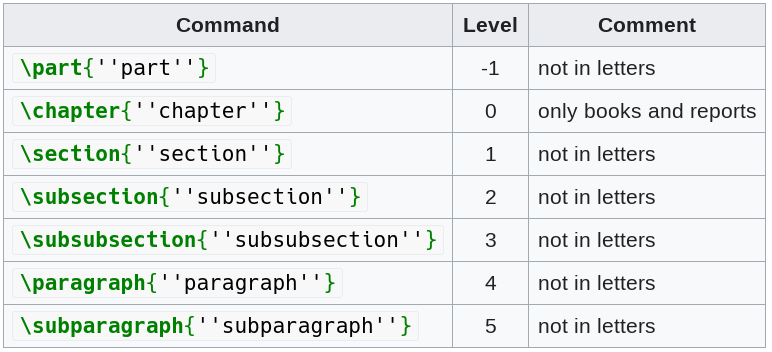
\includegraphics[width=0.63\textwidth, height=0.53\textheight]{docs/images/sections} 
\end{center}
\end{itemize}
\end{frame}

\begin{frame}{نمونه‌های تگ‌های ساختاربندی}
\begin{itemize}\itemr
\item[]
\begin{center}
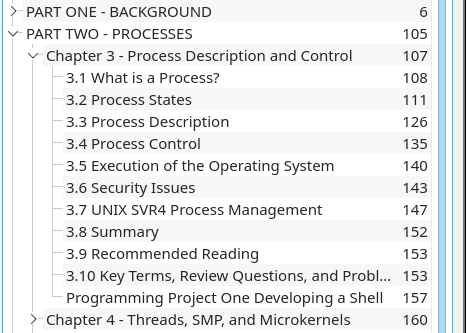
\includegraphics[width=0.5\textwidth, height=0.6\textheight]{docs/images/secexample}
\end{center}
\end{itemize}
\end{frame}

\begin{frame}[fragile]{نمونه کد}
\begin{latin}
\begin{lstlisting}[keywords={part, chapter, section, subsection}, keywordstyle=\color{Mulberry}\textbf]
\begin{document}
\chapter{History}

\section{Creation}

\subsection{Who}
Donald Knuth

\subsection{When}
1978; 45 years ago
\end{document}
\end{lstlisting}
\end{latin}
\end{frame}

\begin{frame}{خروجی}
\begin{center}
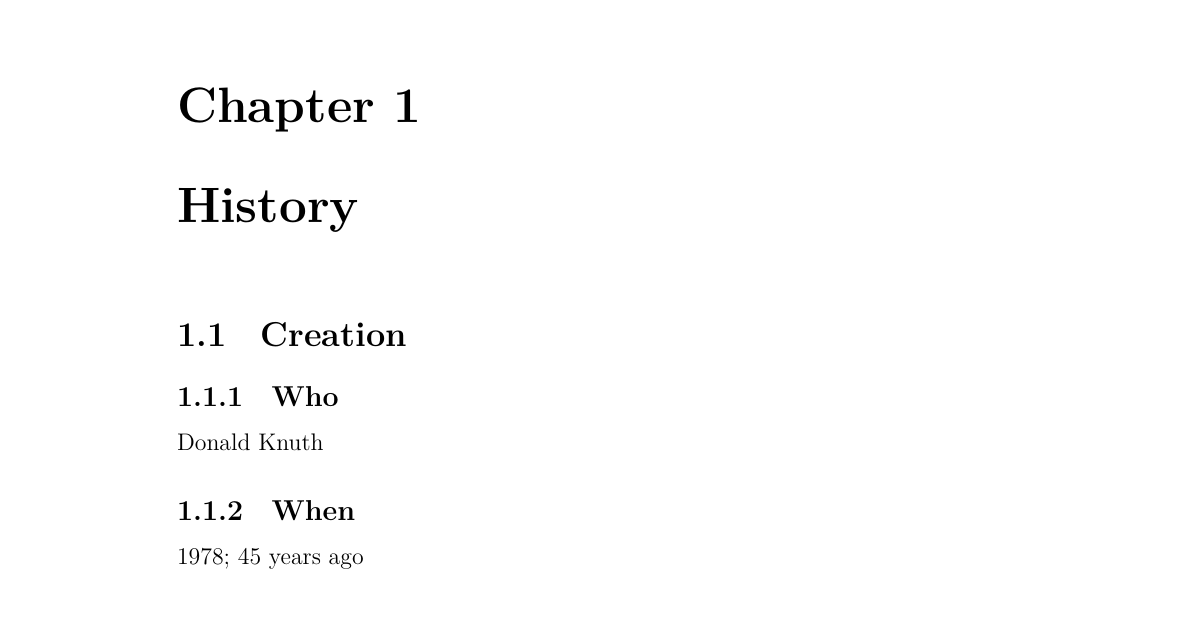
\includegraphics[width=0.7\textwidth, height=0.6\textheight]{docs/images/chsec}
\end{center}
\end{frame}

\begin{frame}{خروجی}
\begin{center}
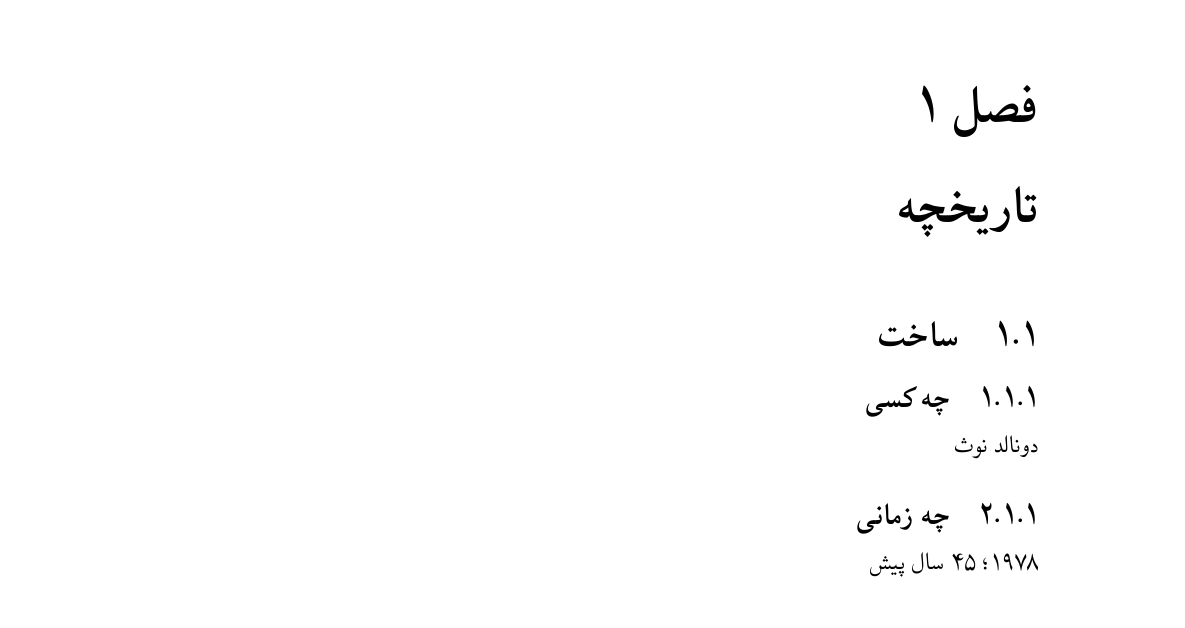
\includegraphics[width=0.7\textwidth, height=0.6\textheight]{docs/images/chsec-fa}
\end{center}
\end{frame}
\section{جداول}

\section{شمارنده‌ها}
\begin{frame}{چرا شمارنده‌ها}
\begin{itemize}\itemr
\item[-]
در نوشتن متون، مواقعی پیش می‌آید که باید به تعداد مشخص یا نامشخصی مواردی را بنویسیم و برای آنها شماره‌گذاری انجام دهیم،

\item[-]
مثل ردیف جدول‌ها.

\item[-]
اما انجام دادن دستی این کار، عدم دقت، ناهماهنگی و زحمت زیادی را برای ما دارد.

\item[-]
راهکار نرم‌افزار لاتک، استفاده از شمارنده‌هاست.
\end{itemize}
\end{frame}

\begin{frame}{استفاده‌ی خود لاتک از شمارنده‌ها}
\begin{itemize}\itemr
\item[-]
لاتک برای شماره‌گذاری صفحات، قسمت‌ها، فصول و سکشن‌ها
(\ref{parts-chapters})،
 و موارد زیاد دیگری از شمارنده‌های درونی خودش استفاده می‌کند.
\end{itemize}
\end{frame}

\begin{frame}[fragile]{نمونه کد}
\begin{latin}
\begin{lstlisting}[keywords={begin, end}, keywordstyle=\color{Mulberry}\textbf]
\LaTeX uses counters for
\begin{enumerate}
    \item \textbackslash part
    \item \textbackslash chapter
    \item \textbackslash section
    \item \textbackslash subsection
\end{enumerate}
\end{lstlisting}
\end{latin}
\end{frame}

\begin{frame}{خروجی}
\begin{center}
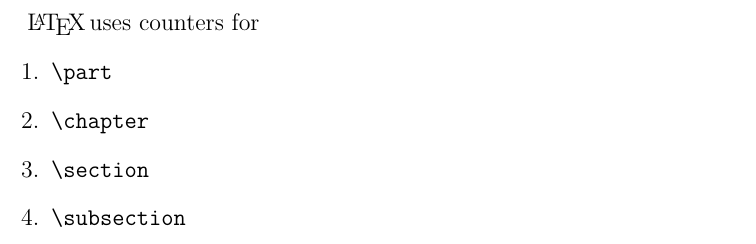
\includegraphics[width=\textwidth]{docs/images/enum-1}
\end{center}
\end{frame}

\begin{frame}[fragile]{نمونه کد}
\begin{latin}
\begin{lstlisting}[keywords={begin, end}, keywordstyle=\color{Mulberry}\textbf]
\LaTeX uses counters for
\begin{enumerate}
    \item even this \texttt{enumerate} environment
    \item \textbackslash part
    \item \textbackslash chapter
    \item \textbackslash section
    \item \textbackslash subsection
\end{enumerate}
\end{lstlisting}
\end{latin}
\end{frame}

\begin{frame}{خروجی}
\begin{center}
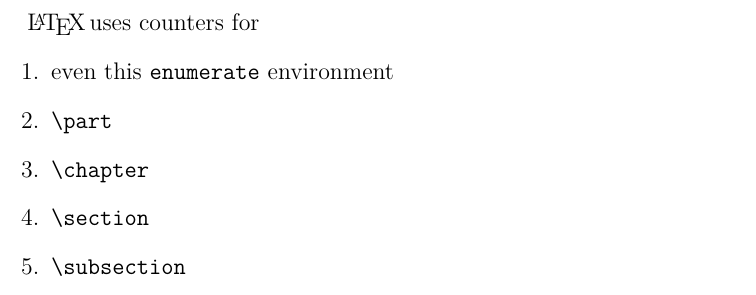
\includegraphics[width=\textwidth]{docs/images/enum-2}
\end{center}
\end{frame}


\begin{frame}{تعریف شمارنده}
\begin{itemize}\itemr
\item[-]
برای تعریف شمارنده‌های باید از دستور
\lr{\texttt{\textbackslash newcounter\{NameOfCounter\}}} 
استفاده کرد.
\end{itemize}
\end{frame}

\begin{frame}{تعریف شمارنده}
\begin{itemize}\itemr
\item[-]
برای دسترسی به مقدار شمارنده، از این سه روش می‌توان استفاده کرد:

\begin{enumerate}\itemr
\item 
\lr{\texttt{\textbackslash theNameOfCounter}}

\item 
\lr{\texttt{\textbackslash value\{NameOfCounter\}}}

\item
\lr{\texttt{\textbackslash arabic\{NameOfCounter\}}}
\end{enumerate}
\end{itemize}
\end{frame}

\begin{frame}{حالت مقدار شمارنده}
\begin{itemize}\itemr
\item[-]
\lr{\texttt{\textbackslash arabic}}

برای مقادیر $-2^{31}$ تا $2^{31}$

\item[-]
\lr{\texttt{\textbackslash alph}}

به ترتیبِ حروف الفبا در انگلیسی و حروف ابجد در فارسی

\item[-]
\lr{\texttt{\textbackslash roman}}

حروف یونانی
\end{itemize}
\end{frame}

\begin{frame}{عدد دهی به شمارنده و گام شمارنده}
\begin{itemize}\itemr
\item[-]
برای مقداردهی به شمارنده (چه به صورت پیشفرض به عدد صفر مقداردهی می‌شوند) از دستور 
\lr{\texttt{\textbackslash setcounter\{NameOfCounter\}\{number\}}}
استفاده می‌شود.

\item[-]
برای گامِ شمارنده، از دستور 
\lr{\texttt{\textbackslash stepcounter\{NameOfCounter\}}}
استفاده می‌شود.
\end{itemize}
\end{frame}

\begin{frame}[fragile]{نمونه کد}
\begin{latin}
\begin{lstlisting}[keywords={begin, end}, keywordstyle=\color{Mulberry}\textbf]
\newcounter{record}
\begin{table}[h]
\begin{tabular}{|c|c|}
\hline
record & course \\
\hline
\hline
\stepcounter{record}\arabic{record} & Operating System \\
\hline
\stepcounter{record}\arabic{record} & Computer Networks \\
\hline
\stepcounter{record}\arabic{record} & Signals and Systems \\
\hline
\stepcounter{record}\arabic{record} & Project Management \\
\hline
\end{tabular}
\end{table}
\end{lstlisting}
\end{latin}
\end{frame}

\begin{frame}{خروجی}
\begin{center}
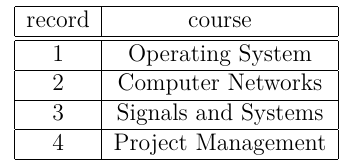
\includegraphics[width=0.5\textwidth]{docs/images/engcounter}
\end{center}
\end{frame}

\begin{frame}{خروجی}
\begin{center}
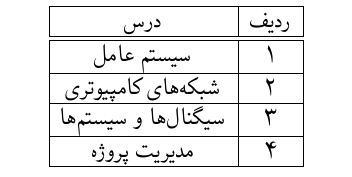
\includegraphics[width=0.5\textwidth]{docs/images/facounter}
\end{center}
\end{frame}

\section{فرمول‌های ریاضی}
\section{ارجاع‌دهی‌‌ها}
\begin{frame}{ارجاع‌دهی‌‌ها در خود سند}
\begin{itemize}\itemr
\item[-]
در مواقع زیادی نیاز به ارجاع‌دهی در قسمت‌ها مختلف سند، احساس می‌شود.
\item[-]
برای مثال برای ارجاع‌دهی به یک فصل خاص، سکشن‌ خاص، جدول و یا تصاویر مختلف نیاز به یک ارجاع‌دهی پویا داریم.

\item[-]
فرض کنید چنین متنی داریم: \textit{با توجه به مباحثی که در فصل ۲ انجام شد...}
و سپس تصمیم می‌گیریم که قبل از فصل ۲، یک فصل دیگر بنویسیم و در واقع فصل ۲، می‌شود فصل ۳.

\item[-]
اگر این ارجاع‌دهی را به صورت دستی انجام داده باشیم، باید بگردیم و تمامی \textit{فصل ۲}‌های داخل متنمان را به \textit{فصل ۳} تغییر بدهیم.

\item[-]
اما، همانند کاری که برای شمارنده‌ها کردیم، میتوانیم از امکانات خود لاتک برای ارجاع‌دهی استفاده کنیم.
\end{itemize}
\end{frame}

\begin{frame}{ارجاع‌دهی‌‌ها در خود سند}
\begin{itemize}\itemr
\item[-]
برای اینکار باید از دو دستور استفاده کنیم:
\begin{enumerate}\itemr
\item 
\lr{\texttt{\textbackslash lable\{UniqueLabel\}}} 
برای نشانه‌گذاری

\item 
\lr{\texttt{\textbackslash ref\{UniqueLable\}}}
برای ارجاع‌دهی 
\end{enumerate}
\end{itemize}
\end{frame}

\begin{frame}[fragile]{نمونه کد}
\begin{latin}
\begin{lstlisting}[keywords={chapter, section, label, ref}, keywordstyle=\color{Mulberry}\textbf]
\chapter{Processes and Threads}
\section{Processes}\label{processes}
\section{Threads}
As mentioned in the \ref{processes},
OS must schedule and dispatch...
\end{lstlisting}
\end{latin}
\end{frame}

\begin{frame}{خروجی}
\begin{center}
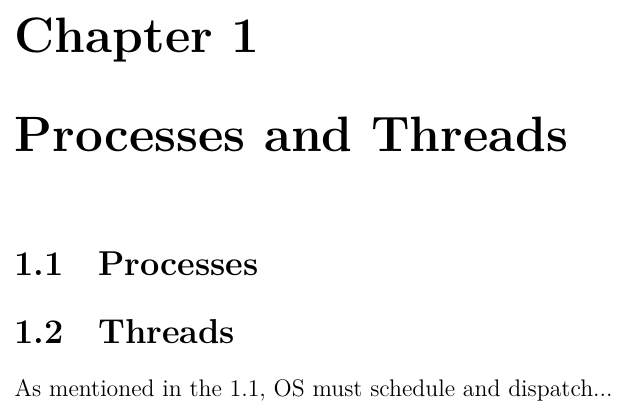
\includegraphics[width=0.65\textwidth, height=0.7\textheight]{docs/images/proc-ref}
\end{center}
\end{frame}


\begin{frame}[fragile]{نمونه کد}
\begin{latin}
\begin{lstlisting}[keywords={chapter, section, label, ref}, keywordstyle=\color{Mulberry}\textbf]
\chapter{Processes and Threads}
\section{Operating System}
\section{Processes}\label{processes}
\section{Threads}
As mentioned in the \ref{processes}, 
OS must schedule and dispatch...
\end{lstlisting}
\end{latin}
\end{frame}

\begin{frame}{خروجی}
\begin{center}
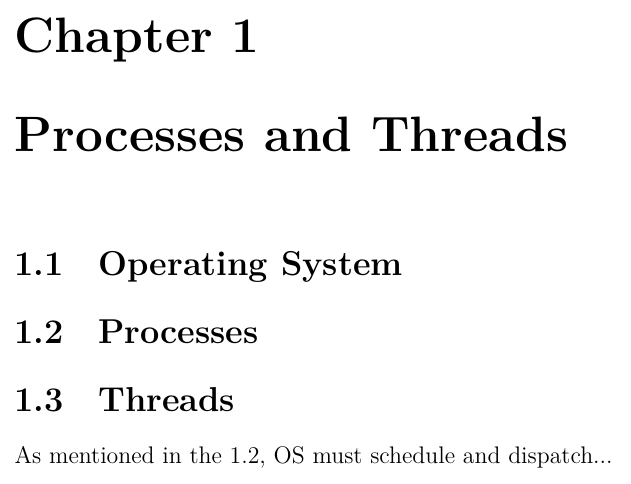
\includegraphics[width=0.55\textwidth, height=0.7\textheight]{docs/images/proc-ref-1}
\end{center}
\end{frame}

\begin{frame}{ارجاع‌دهی‌‌ها در خود سند}
\begin{itemize}\itemr
\item[-]
حتی می‌توان بجای ارجاع‌دهی با عدد، با نام هم به مطلب مورد نظر، ارجاع داد.

\item[-]
برای این کار باید از بسته‌ی 
\lr{\texttt{nameref}}
و تگ
\lr{\texttt{\textbackslash nameref\{UniqueLable\}}}
استفاده کرد.
\end{itemize}
\end{frame}

\begin{frame}[fragile]{نمونه کد}
\begin{latin}
\begin{lstlisting}[keywords={chapter, section, label, ref}, keywordstyle=\color{Mulberry}\textbf]
\chapter{Processes and Threads}
\section{Processes}\label{processes}
\section{Threads}
As mentioned in the \nameref{processes},
OS must schedule and dispatch...
\end{lstlisting}
\end{latin}
\end{frame}

\begin{frame}{خروجی}
\begin{center}
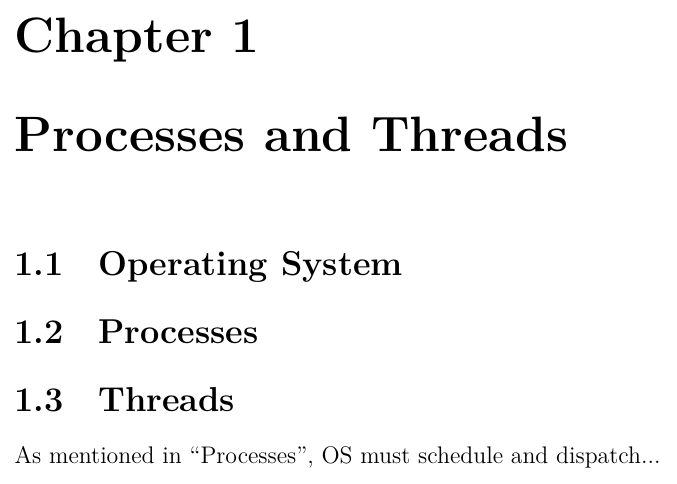
\includegraphics[width=0.55\textwidth, height=0.7\textheight]{docs/images/proc-nameref}
\end{center}
\end{frame}

\begin{frame}[fragile]{نمونه کد}
\begin{latin}
\begin{lstlisting}[keywords={chapter, section, label, ref}, keywordstyle=\color{Mulberry}\textbf]
\chapter{Processes and Threads}
\section{What Are Processes?}\label{processes}
\section{Threads}
As mentioned in the \nameref{processes},
OS must schedule and dispatch...
\end{lstlisting}
\end{latin}
\end{frame}

\begin{frame}{خروجی}
\begin{center}
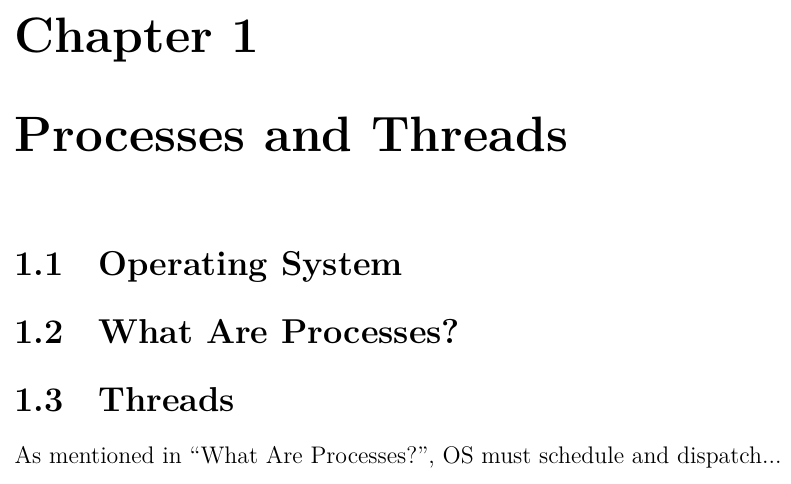
\includegraphics[width=0.7\textwidth, height=0.75\textheight]{docs/images/proc-nameref-change}
\end{center}
\end{frame}

\section{انواع فهرست‌ها}
\begin{frame}{فهرست‌ها}
\begin{itemize}\itemr
\item[-]
یکی از وابسته‌های نوشتاری بسیار مورد نیاز، تولید انواع فهرست‌هاست.

\item[-]
فهرست مطالب، فهرست عکس‌ها و فهرست جداول از فهرست‌های متداول در متون هستند.

\item[-]
نوشتن دستی فهرست‌ها از سخت‌ترین، پر غلط‌ترین و حوصله‌ سربرترین کار‌هاست.

\item[-]
به همین جهت، لاتک تگ‌هایی در اختیار ما قرار داده است که به آسان‌ترین، صحیح‌ترین و جذاب‌ترین روش این فهرست‌ها را تولید کنیم.
\end{itemize}
\end{frame}

\begin{frame}{فهرست مطالب}
\begin{itemize}\itemr
\item[-]
یکی از اصلی‌ترین فهرست‌ها، فهرست مطالب سند است.

\item[-]
برای تولید فهرست مطالب کافی‌ست که از دستور 
\lr{\texttt{\textbackslash tableofcontents}}
استفاده کرد.
\end{itemize}
\end{frame}

\begin{frame}[fragile]{نمونه کد}
\begin{latin}
\begin{lstlisting}[keywords={begin, end}, keywordstyle=\color{Mulberry}\textbf]
\begin{document}
\tableofcontents

\part{Intro}
\chapter{\LaTeX}
\section{What is \TeX}
\section{Why \LaTeX}

\chapter{Who created \LaTeX}

\part{Main}
\chapter{Structuring}
\chapter{Tables}
\section{\texttt{\textbackslash table} Environment}
\section{\texttt{\textbackslash tabular} Environment}
\section{Aligning Columns}
\end{document}
\end{lstlisting}
\end{latin}
\end{frame}

\begin{frame}{خروجی}
\begin{center}
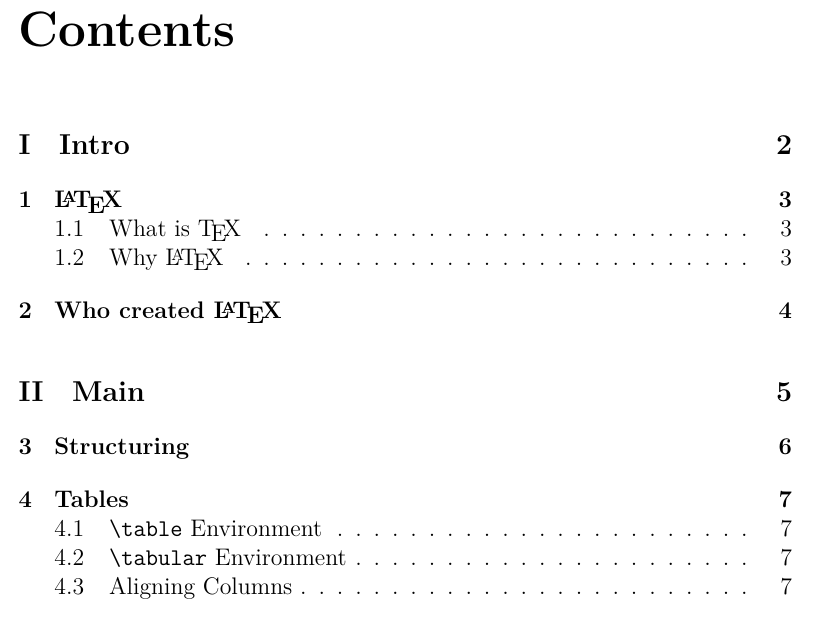
\includegraphics[width=0.7\textwidth, height=0.8\textheight]{docs/images/tab-cont}
\end{center}
\end{frame}

\begin{frame}{لینک کردن}
\begin{itemize}\itemr
\item[-]
یکی دیگر از قابلیت‌های بسیار جذاب لاتک، درست کردن لینک برای فهرست‌ها و همچنین ارجاع‌دهی‌هاست.

\item[-] 
تمام این کار توسط لاتک انجام شده و روی فایل \lr{pdf} خروجی اعمال می‌شود و تنها کار مورد نیاز ما استفاده از بسته 
\lr{\texttt{hyperref}}
است.
\end{itemize}
\end{frame}

\begin{frame}[fragile]{نمونه کد}
\begin{latin}
\begin{lstlisting}[keywords={begin, end}, keywordstyle=\color{Mulberry}\textbf]
\usepackage{hyperref}

\begin{document}
...
\end{document}
\end{lstlisting}
\end{latin}
\end{frame}

\begin{frame}{خروجی}
\begin{center}
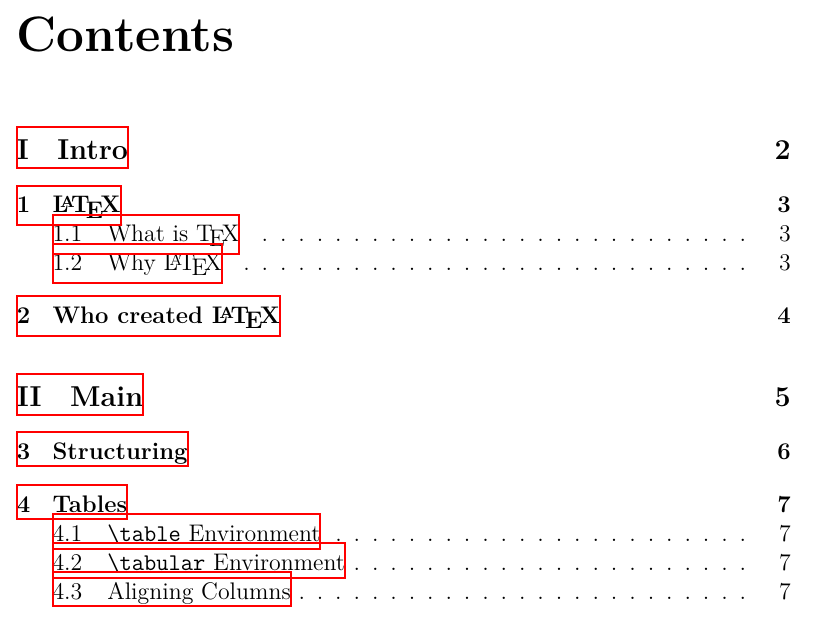
\includegraphics[width=0.7\textwidth, height=0.8\textheight]{docs/images/hyperref-simple}
\end{center}
\end{frame}

\begin{frame}{خروجی}
\begin{center}
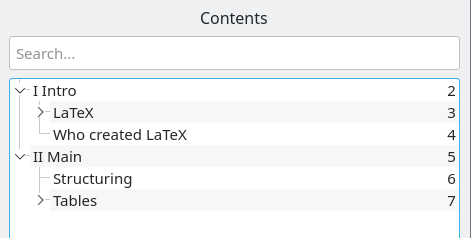
\includegraphics[width=0.5\textwidth, height=0.5\textheight]{docs/images/hyperref-affect}
\end{center}
\end{frame}

\begin{frame}{بسته \lr{\texttt{hyperref}}}
\begin{itemize}\itemr
\item[-]
مشاهده‌ کردید که تنها با استفاده از این بسته، چنین تغییراتی روی متن و فایل \lr{pdf} خروجی رخ داد.

\item[-]
اما این حالت پیش‌فرض کمی (کم نه، خیلی زیاد) زشت و ناجور است.

\item[-]
براحتی می‌توان خروجی این بسته را ویرایش کرد و به نتیجه‌ی دلخواه رسید.
\end{itemize}
\end{frame}

\begin{frame}[fragile]{نمونه کد}
\begin{latin}
\begin{lstlisting}[keywords={begin, end}, keywordstyle=\color{Mulberry}\textbf]
\usepackage{hyperref}
\hypersetup{
    colorlinks=true,
    linkcolor=blue,
    filecolor=magenta,      
    urlcolor=blue,
}

\begin{document}
...
\end{document}
\end{lstlisting}
\end{latin}
\end{frame}

\begin{frame}{خروجی}
\begin{center}
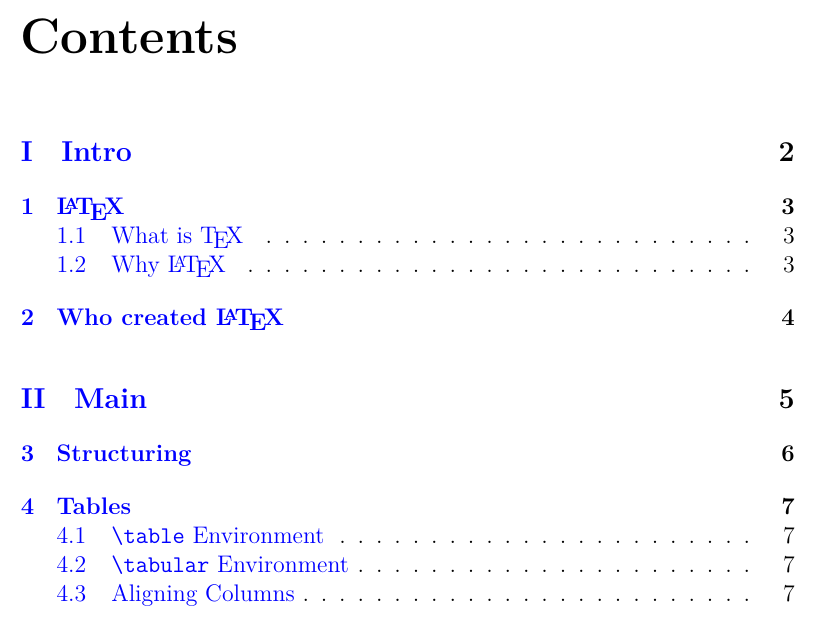
\includegraphics[width=0.7\textwidth, height=0.8\textheight]{docs/images/hyperref-edited}
\end{center}
\end{frame}


\begin{frame}{دیگر فهرست‌ها}
\begin{itemize}\itemr
\item[-]
برای تولید فهرست عکس‌ها، باید توجه داشته باشید که عکس‌ها را باید در محیط 
\lr{\texttt{figure}}
گذاشت و سپس از دستور 
\lr{\texttt{\textbackslash listoffigures}}
استفاده کرد.

\item[-]
برای تولید فهرست جداول نیز از دستور 
\lr{\texttt{\textbackslash listoftables}}
استفاده می‌شود.
\end{itemize}
\end{frame}

\section{شعر‌ فارسی}
\begin{frame}{نوشتن شعر فارسی}
\begin{itemize}\itemr
\item[-]
نوشتن شعر فارسی هم به راحتی نوشتن دیگر امکانات لاتک است.

\item[-]
برای نوشتن شعر فارسی باید از بسته 
\lr{\texttt{bidipoem}}
و محیط 
\lr{\texttt{traditionalpoem}}
استفاده کرد.
\end{itemize}
\end{frame}

\begin{frame}[fragile]{نمونه کد}
\begin{center}
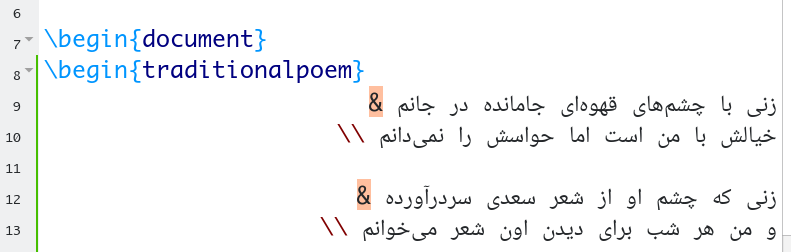
\includegraphics[width=\textwidth]{docs/images/tradpoem-code}
\end{center}
\end{frame}

\begin{frame}{خروجی}
\begin{center}
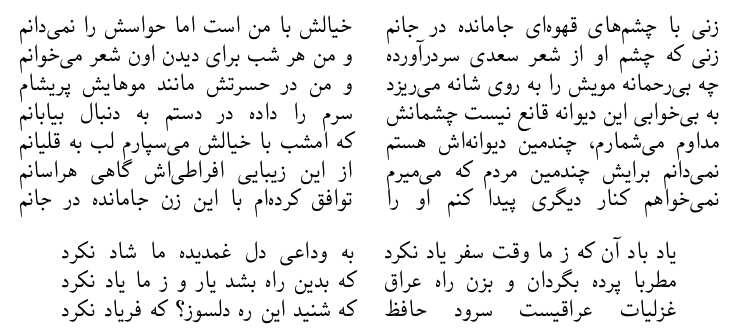
\includegraphics[width=\textwidth]{docs/images/tp-2}
\end{center}
\end{frame}

\end{document}
